\section{Beam Deflection}

\textbf{Goal:} Determine the deflection and slope at specified points of beams and shafts

\vspace{5pt}

\noindent \textbf{Solve statically indeterminate beams:} where the number of reactions at the supports exceeds the number of equilibrium equations available.

\vspace{5pt}

\noindent \textbf{Maximum deflection of the beam:} Design specifications of a beam will generally include a maximum allowable value for its deflection.

\vspace{5pt}

\subsection{Sign Conventions}

\begin{figure*}[!h]
\centering
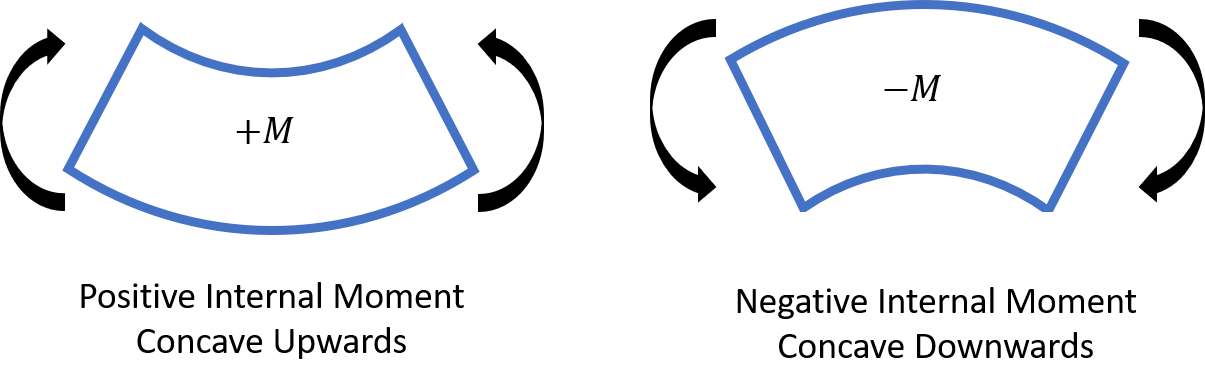
\includegraphics[angle=0, width=4in]{Beam Deflection-Figures/signConvention1.png}
\vspace{-2mm}
\caption{\small From ref pages}
\vspace{-3mm}
\label{Fig:Signs}
\end{figure*}

\subsection{Boundary Conditions}

\begin{figure*}[!h]
\centering
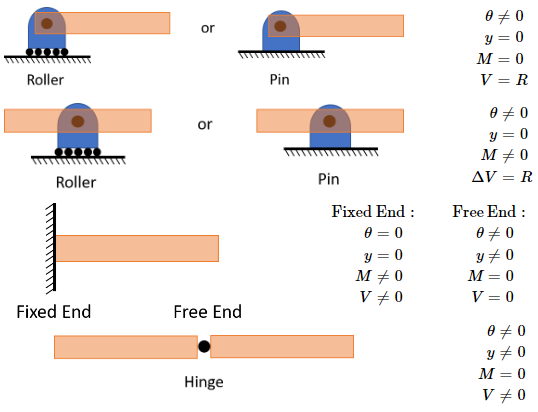
\includegraphics[angle=0, width=4in]{Beam Deflection-Figures/BoundryConditions.png}
\vspace{-2mm}
\caption{\small From ref pages}
\vspace{-3mm}
\label{Fig:Boundaries}
\end{figure*}


\subsection{\blue{Moment-Curvature Equation}}

\noindent \textbf{Elastic Curve of a Beam:} 

\begin{figure*}[!h]
\centering
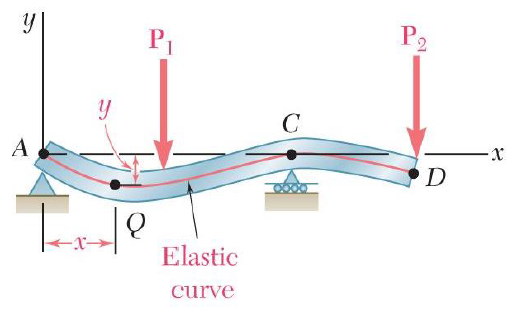
\includegraphics[angle=0, width=2.5in]{Beam Deflection-Figures/ElasticCurveBeam.png}
\vspace{-2mm}
\caption{\small \blue{Taken from TAM251 Lecture Notes - L12S3}}
\vspace{-3mm}
\label{Fig:ElasticCurveBeam}
\end{figure*}

\noindent Moment-curvature equation:
 
\[M(x) = \frac{E(x)I(x)}{\rho(x)}\]
\[\kappa = \frac{1}{\rho} = \frac{M(x)}{EI}\]

\begin{figure*}[!h]
\centering
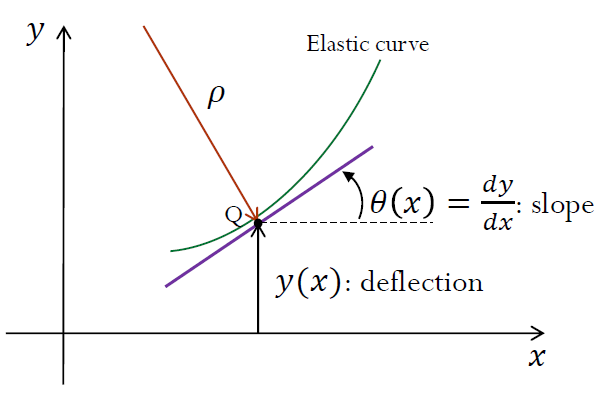
\includegraphics[angle=0, width=3in]{Beam Deflection-Figures/ElasticCurveGraph.png}
\vspace{-2mm}
\caption{\small \blue{Taken from TAM251 Lecture Notes - L12S3}}
\vspace{-3mm}
\label{Fig:ElasticCurvegraph}
\end{figure*}

\noindent Governing equation of the elastic curve:
\[\frac{d^2y}{dx^2} = \frac{M(x)}{EI}\]




\subsubsection{\blue{Assumptions}}

\blue{
\begin{itemize}
    \item $y(x)$ is the vertical direction
    \item Bending only: we will neglect effects of transverse shear
    \item Small deflection angles 
\end{itemize}
}

\subsection{\blue{Integration Methods}}

\noindent Elastic curve equation for constant $E$ and $I$: $EIy'' = M(x)$

\vspace{5pt}

\noindent Differentiating both sides gives: $EIy''' = \frac{dM(x)}{dx} = V(x)$

\vspace{5pt}

\noindent Differentiating again: $EIy'''' = \frac{dV(x)}{dx} = w(x)$ 

\vspace{5pt}

\noindent In summary, we have:

\[V(x) = \int w(x) dx\]
\[M(x) = \int V(x)dx\]
\[\frac{dy}{dx} = \int \frac{1}{EI}M(x)dx\]
\[y(x) = \int y'(x) dx\]

\vspace{5pt}

\noindent Where:

\vspace{5pt}

\noindent $y(x):$ deflection

\vspace{5pt}

\noindent $y'(x):$ slope

\vspace{5pt}

\noindent $EIy''(x):$ bending moment

\vspace{5pt}

\noindent $EIy'''(x):$ shear force

\vspace{5pt}

\noindent $EIy''''(x):$ distributed load

\clearpage

\noindent \textbf{Example:} Overhanging Beam

\begin{figure*}[!h]
\centering
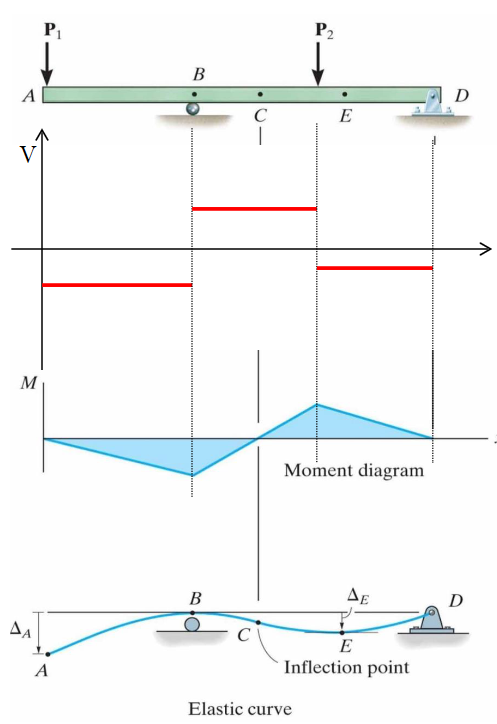
\includegraphics[angle=0, width=3in]{Beam Deflection-Figures/Overhang Ex.png}
\vspace{-2mm}
\caption{\small \blue{Taken from TAM251 Lecture Notes - L12S8}}
\vspace{-3mm}
\label{Fig:OverhangEx}
\end{figure*}

\noindent \textbf{Example:} Cantilever Beam

\begin{figure*}[!h]
\centering
\includegraphics[angle=0, width=3in]{Beam Deflection-Figures/cantilever Ex.png}
\vspace{-2mm}
\caption{\small \blue{Taken from TAM251 Lecture Notes - L12S8}}
\vspace{-3mm}
\label{Fig:CantileverEx}
\end{figure*}

\clearpage

\subsection{\blue{Beam Solutions}}

\blue{Common beam deflection solutions have been worked out.}

\begin{figure*}[!h]
\centering
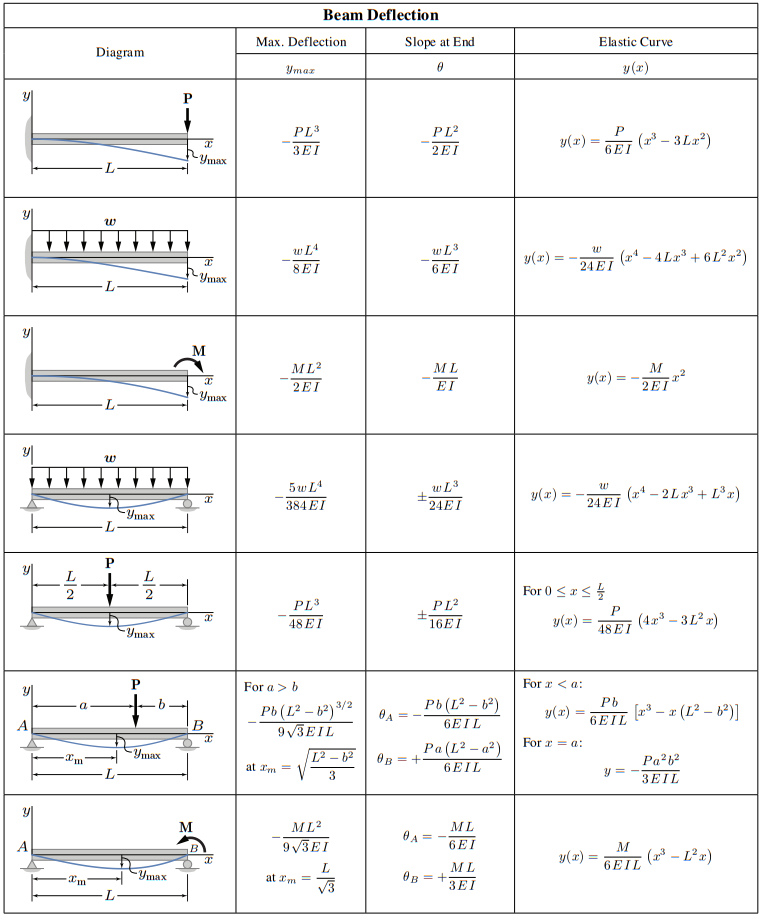
\includegraphics[angle=0, width=\columnwidth]{Beam Deflection-Figures/Common Solutions.png}
\vspace{-2mm}
\caption{\small \blue{Taken from the formula sheet}}
\vspace{-3mm}
\label{Fig:CommonSolutions}
\end{figure*}

\clearpage

\noindent \blue{To solve loadings that are not in the table, use \textbf{superposition} to get the resulting deflection curve.} 

\vspace{5pt}

\noindent \blue{\textbf{Example:} Moment and distributed load}

\begin{figure*}[!h]
\centering
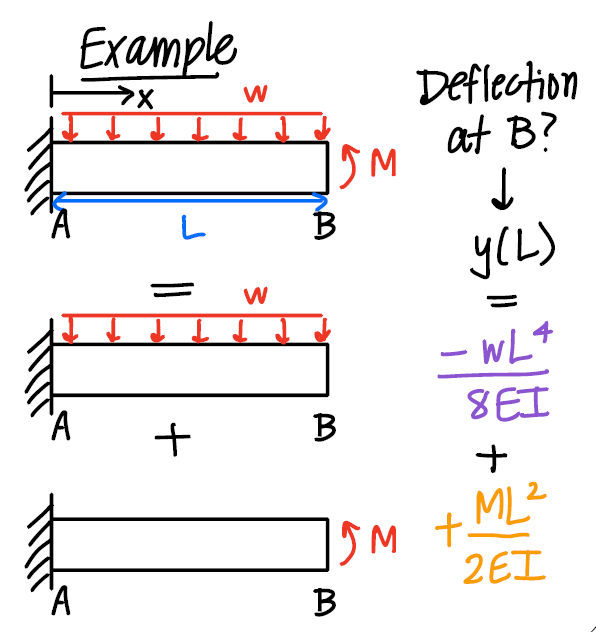
\includegraphics[angle=0, width=3in]{Beam Deflection-Figures/Superposition Ex.png}
\vspace{-2mm}
\caption{\small \blue{Taken from TAM251 Lecture Notes - L12S16}}
\vspace{-3mm}
\label{Fig:SuperpositionEx}
\end{figure*}